\documentclass[]{standalone}
\usepackage{tikz}
\usetikzlibrary{shapes,arrows,calc,positioning}
\usepackage{amsmath} % for dfrac
\usepackage{comment}
\usepackage{calc}

% definition of basic block
\tikzset{
    block/.style = {draw, rectangle,
        minimum height=1.2cm,
        minimum width=2cm},
    input/.style = {coordinate,node distance=1cm},
    output/.style = {coordinate,node distance=1cm},
    sum/.style = {draw, circle, node distance=1cm},
}

% definition of saturation block
\tikzset{% from https://tex.stackexchange.com/questions/161075/saturation-block
  saturation block/.style={%
    draw, 
    path picture={
      % Get the width and height of the path picture node
      \pgfpointdiff{\pgfpointanchor{path picture bounding box}{north east}}%
        {\pgfpointanchor{path picture bounding box}{south west}}
      \pgfgetlastxy\x\y
      % Scale the x and y vectors so that the range
      % -1 to 1 is slightly shorter than the size of the node
      \tikzset{x=\x*.4, y=\y*.4}
      %
      % Draw annotation
      \draw (-1,0) -- (1,0) (0,-1) -- (0,1); 
      \draw (-1,-.7) -- (-.6,-.7) -- (.6,.7) -- (1,.7);
    }
  }
}
\tikzset{% from https://tex.stackexchange.com/questions/161075/saturation-block
  deadband block/.style={%
    draw, 
    path picture={
      % Get the width and height of the path picture node
      \pgfpointdiff{\pgfpointanchor{path picture bounding box}{north east}}%
        {\pgfpointanchor{path picture bounding box}{south west}}
      \pgfgetlastxy\x\y
      % Scale the x and y vectors so that the range
      % -1 to 1 is slightly shorter than the size of the node
      \tikzset{x=\x*.4, y=\y*.4}
      %
      % Draw annotation
      \draw (-1,0) -- (1,0) (0,-1) -- (0,1);  % axis
      \draw (-1,1) -- (-.3,.3) -- (-.3,0) -- (.3,0) -- (.3,-.3) -- (1,-1);
	  %\draw (-.3,.3) -- (.3,-.3) ;
    }
  }
}

\begin{document}
	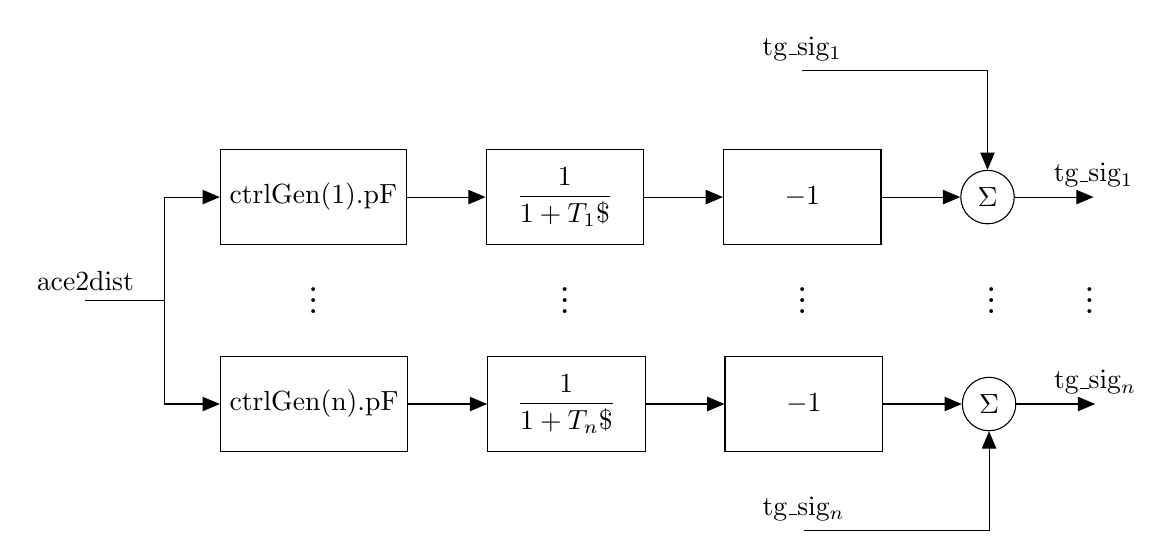
\begin{tikzpicture}[auto, node distance=1cm,>=triangle 45]
	% star input
	\node [input, name=ace2distIn, label=ace2dist] {};
	\coordinate [right=of ace2distIn]  (inputSpace) {};
	
	% pf gain
	\node [block, above right=of inputSpace, name=gen1Pf] {ctrlGen(1).pF};
	\node [input, below=of gen1Pf, label=\Large \vdots]  (dots1) {};
	\node [block, below right=of inputSpace, name=gennPf] {ctrlGen(n).pF};
	
	% filter
	\node [block, right=of gen1Pf, name=gen1lp] {$\dfrac{1}{1+T_1\$}$};
	\node [input, below=of gen1lp, label=\Large \vdots]  (dots2) {};
	\node [block, right=of gennPf, name=gennlp] {$\dfrac{1}{1+T_n\$}$};
	
	% gain
	\node [block, right=of gen1lp, name=gain1] {$-1$};
	\node [input, below=of gain1, label=\Large \vdots]  (dots3) {};
	\node [block, right=of gennlp, name=gain2] {$-1$};
	
	%sum
	\node [sum, right=of gain1, name=sum1] {$\Sigma$};
	\node [input, right=2.4cm of dots3, label=\Large \vdots]  (dots5) {};
	\node [sum, right=of gain2, name=sum2] {$\Sigma$};
	
	%tg input
		\node [input, above=of gain1, name=tgIn1 , label=tg\_sig$_1$] {};
		\node [input, below=of gain2, name=tgIn2, label=tg\_sig$_n$] {};
	
	%output
	\node [output, right=of sum1, name=out1, label=tg\_sig$_1$] {};
	\node [input, right=1.25 cm of dots5, label=\Large \vdots]  (dots6) {};
	\node [output, right=of sum2, name=out2, label=tg\_sig$_n$] {};
	
	%%lines
	\draw [-] (ace2distIn) -- (inputSpace); 
	\draw [->] (inputSpace) |- (gen1Pf); 
	\draw [->] (inputSpace) |- (gennPf); 
	\draw [->] (gen1Pf) -- (gen1lp); 
	\draw [->] (gennPf) -- (gennlp); 
	\draw [->] (gen1lp) -- (gain1); 
	\draw [->] (gennlp) -- (gain2); 
	\draw [->] (gain1) -- (sum1); 
	\draw [->] (gain2) -- (sum2);
	\draw [->] (tgIn1) -| (sum1); 
	\draw [->] (tgIn2) -| (sum2);
	\draw [->] (sum1) -- (out1); 
	\draw [->] (sum2) -- (out2); 
	\end{tikzpicture} 
\end{document}